\chapter{Radio astronomy}

\section{Introduction}


Modern-day astronomy is at an unprecedented stage, with a deluge of data from different telescopes. In contrast
to conventional methods, today astronomical discoveries are data- driven. The upcoming Square Kilometer Array (SKA) is expected to produce terabytes of data every hour \citep{skatelescope}. With this exponential growth of data, challenges for data calibration, reduction and analysis also increase, making it difficult for astronomers to manually process and analyse the data. Therefore, intelligent and automated systems are required  to overcome these challenges.

One of the main issues in radio astronomy is determining the quality of observational data. Astronomical signals are very weak  by the time they reache the Earth’s surface. They are easily corrupted by atmospheric interferences, incorrect observational parameters (e.g. telescope locations or telescope pointing parameters), malfunctioning signal receivers, interference from terrestrial man-made radio sources and tracking inaccuracies \citep{taylor1999synthesis}. Therefore, it is required to do proper corrections to the observational data before processing the data. Radio astronomers spend a considerable amount of time performing a series of preprocessing steps called $\textit{calibration}$, which involves the determination of a set of parameters to correct the received data. These generally include instrumental as well as astronomical parameters. The general strategy for doing these corrections makes use of a calibrator source. Calibrator sources are well suited for determining astronomical parameters for data corrections because they have known characteristics such as the brightness, shape, and frequency spectrum \citep{taylor1999synthesis}. This process of calibration is iterative and time-consuming.

During scientific observations, different external parameters such as atmospheric pressure, temperature  wind conditions, and relative humidity  are collected through thousands of sensors attached to the telescopes and its adjoining instrumentation. The data coming from different sensors may provide information about the external conditions that may have corrupted the observed data. This piece of information is not always included in the conventional calibration steps. We propose to use machine learning methods to predict the calibration solutions, looking at pointing and environmental sensor data. This is mainly motivated by the fact that calibration steps make corrections to data that have been corrupted by environmental parameters.

In this project, we make use of data from the Karoo Array Telescope (KAT-7), an array consisting of seven telescopes, which is a precursor to the MeerKAT radio telescope. We look at pointing azimuth, elevation, scan, offset, temperature, wind speed, air pressure and relative humidity sensor data recorded during observations with a calibrator source PKS1613-586 to generate the training and testing dataset. The overall generated dataset contains sensor data per telescope and calibration solutions for package the signal received by each telescope in horizontal polarization (H-pol)  and vertical polarization (V-pol). These calibrator solutions are calculated using the astronomy software called Common Astronomy Software Applications (CASA), the popular which is used for data calibration and imaging in radio astronomy.
 
\section{Introduction to radio astronomy}

Radio astronomy is one of the most fascinating fields of study about the Universe. Astronomers capture and analyze the electromagnetic signals emitted by distant objects, such as stars and galaxies, using a radio telescope. In Section \ref{Ra} we present a brief introduction to radio astronomy, including interferometry vs single dish in Section \ref{RvI}. In Section \ref{Calibr} we define calibration in radio astronomy and describe the different techniques used for data calibration in Section \ref{caltech}.
\label{Ra}
\subsection{History}


Radio astronomy is the study of celestial sources emitting radio waves \citep{verschuur2015invisible}. A wave is an oscillatory motion of any kind, the most familiar ones being sound waves and vibrations of various material substances and waves on the surface of water. There are also wave  disturbances found in electric and magnetic field. Such waves are responsible for what we experience daily, i.e. X-rays, visible light, or radio waves \citep{cassidy2002wave}. Traditional astronomy is based on visible light (i.e. optical observations) wavelengths, but astronomical sources emit radiation not only as visible light but
also across the electromagnetic spectrum from gamma rays at short wavelength$(\lambda)$ to radio at long wavelength (low frequency), as shown in Figure \ref{images/Electromagnetic-Spectrum.png} \citep{staats2016genetic}.

\begin{figure}[h!]
  \centering
    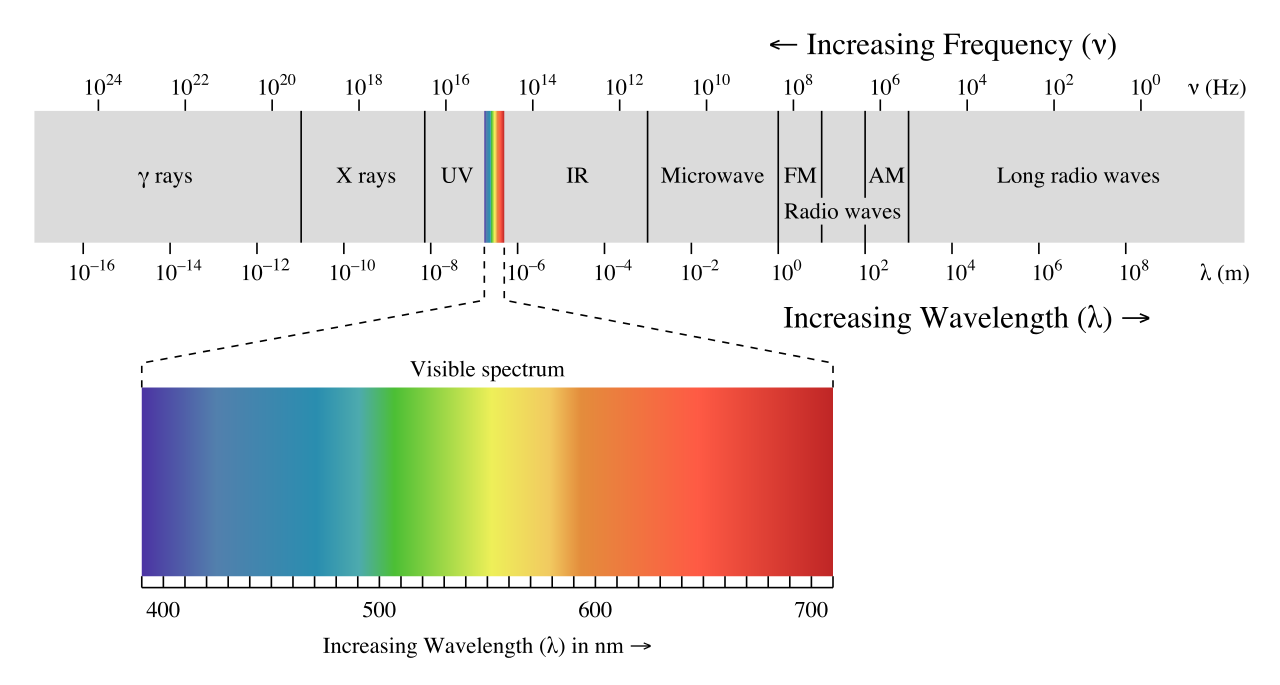
\includegraphics[width=0.7\textwidth]{images/Electromagnetic-Spectrum.png}
    \caption{The electromagnetic spectrum \citep{ElectromagneticSpectrum}}
  \label{images/Electromagnetic-Spectrum.png}
\end{figure}

Electromagnetic radiation is a group of waves created by fluctuations of electric and magnetic fields propagating through space at the speed of light ($c=3\times 10^{8} m/s$) carrying electromagnetic radiant energy \citep{ElectromagneticSpectrum}.\;There are numerous emission mechanisms in the universe that generate radio waves.
Each portion of the electromagnetic spectrum reveals a unique view of the universe and so modern astronomy employs various instruments to look at each portion of the spectrum.\;The Earth's atmosphere absorbs electromagnetic radiation at most infra-red, ultraviolet, X-ray, and gamma-ray wavelengths. This means one can only observe the Universe from the ground in two windows namely the radio and visible wavebands. Radio waves can reveal objects that do not radiate in other parts of the electromagnetic spectrum, and they are able to pass through galactic dust clouds that blocks the view in the optical range and can penetrate the Earth's atmosphere (subject to some limits depending on frequency) \citep{thompson2001interferometry}. After received by a radio telescope, the data are amplified and transferred to a computer for further  data processing, which is discussed in the next chapter.


Radio astronomy was discovered accidentally by a radio engineer, Karl Jansky, in the 1930s.
Jansky was assigned the task of investigating sources of radio interference radio-telephone communication system at short wavelengths (10-20 meters) \citep{verschuur2015invisible}.
The purpose of this task was to determine the direction of the radio wave interference so they could easily tune out the interference by using directional antennas pointed away from the direction of the interference. In the process of conducting this task, Jansky constructed an antenna designed to receive radio waves at a frequency of 20.5 MHz \citep{Jansky0}. The antenna was mounted on a circular train track so that it could be rotated in all possible angles along the ground and could detect radio signal in all possible directions. After several months of recording and analysing the radio signals from all directions, Jansky's investigation was successful and he identified two known signals (from local and  distant thunderstorms), which were interfering with the radio-telecommunication system, and one unknown signal (faint steady hiss). Jansky continued to investigate the unknown signal for over a year and eventually found out that the radiation was coming from the Milky Way. The signal was the strongest in the direction of the center of the Milky Way
galaxy, in the constellation of Sagittarius. This was the first detection of non-black body radiation at radio wavelengths from an extraterrestrial source. Black body radiation is the radiation given off by any object
related to its temperature \citep{Jansky1}.

After Jansky's project at Bell Laboratory ended, Bell was not interested in studying astronomy any more. In 1937, an astronomer, Grote Reber, who was fascinated by Jansky's ground-breaking discovery, decided to continue where Jansky had left off by further investigating the cosmic radio waves from the Milky Way galaxy. To pursue this research, Reber built the first single-dish radio telescope with a receiver strong enough to detect cosmic radio signals in his backyard. He spent hours at night scanning the sky at different frequencies. He was finally successful at detecting radio emission from the Milky Way galaxy, confirming Jansky's discovery \citep{verschuur2015invisible}.   

Astronomical signals tend to be weak by the time they reach the ground. The need for greater sensitivity and higher resolution has resulted in the creation of telescopes that have a larger collecting area for more radio energy to be focused on the receiver \citep{verschuur2015invisible}. However, constructing a single-dish telescope large enough i.e. $>500\;m$ to achieve high angular resolution $\theta \approx\frac{\lambda}{D}$ (where $\lambda$ is the wavelength of the electromagnetic radiation observed and $D$ is the aperture diameter of the radio telescope), is physically impossible owing to the cost of the materials and the structure being at high risk to collapsing during high wind conditions. The angular resolution of a radio telescope measures its ability to detect fine details in the structure of the observed celestial source. For example, to obtain an angular resolution of 1 arc-second, would require a single-dish radio telescope's diameter to be thousands of metres \citep{verschuur2015invisible}. 

\section{Single dish vs interferometry}
\label{RvI}


A single-dish survey can be complemented by an array of small radio telescopes providing higher sensitivity and higher resolution images  \citep{thompson2001interferometry}. This technique is called radio interferometry. Radio interferometry is mostly used to obtain high resolution images of astronomical sources, where-as a single-dish technique is mostly considered as a tool for low spacial resolution, i.e., it allows for imaging of very large sources \citep{thompson2001interferometry}. Though these two techniques are quite different, they both provide measurements of the Fourier transform of  some region in the sky \citep{cornwell1988radio}. In this dissertation we focus on the interferometer, which consists of two or more sub-apertures grouped together to form a large array \citep{verschuur2015invisible}, as shown in Figure \ref{images/Rint.png}. Though the telescopes are placed at different positions separated by distance $b$, the resulting power output from all the telescopes is combined. For an interferometric array, the angular resolution is defined as  $\theta \approx\frac{\lambda}{B}$, where $B$ represents the t maximum baseline in the array. 

\begin{figure}[h!]
  \centering
    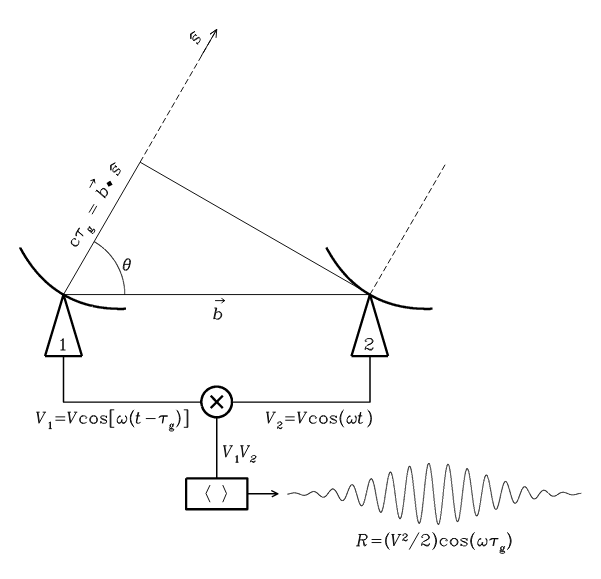
\includegraphics[width=0.45\textwidth]{images/Rint.png}
    \caption{Two-antenna interferometer diagram [National Radio Astronomy Observatory]}
  \label{images/Rint.png}
\end{figure}

Figure \ref{images/Rint.png} illustrates a simple two two-element interferometer consisting of baseline $\overrightarrow{b}$ (we will refer to the left antenna as antenna 1 and the right antenna as antenna 2). This can be extended to multi-antenna arrays by adding more $N$ antennas in the array such that the number of baselines  $\frac{N(N-1)}{2}$  increases \citep{thompson2001interferometry}. From Figure \ref{images/Rint.png}, suppose a distant source is observed in the direction $\widehat{s}$, the incoming signal will arrive in each radio telescope at slightly  different times. To compensate for this time difference such that the signal arrives in each telescope at the same time, a time delay term $\tau_{g}=\frac{\overrightarrow{b}\cdot\widehat{s}}{c}$ is introduced to produce voltages $V_1$ and $V_2$ from antenna 1 and antenna 2 denoted by: 

\begin{equation}\label{eq111}
\begin{split}
V_1(t)&=V\cos[\omega(t-\tau_{g})],\; \text{where} \;\nu=\frac{\omega}{2\pi}\; \text{is the center frequency} \\
V_2(t)&=V\cos(\omega\tau_{g}).
\end{split}
\end{equation}

The inputs $V_1$ and $V_2$ in to the correlator are then  multiplied and time averaged to yield an output response of  amplitude $R$ which is proportional to the point-source flux density and with its phase depending on the time delay and the frequency.

\begin{align}
V_1 \times V_2 = V^2 \cos(\omega\tau_{g})\times \cos[\omega(t-\tau_{g})]
\end{align}
From $\cos A\cos B= \frac{1}{2} \left(\cos (A+B) + \cos (A-B) \right)$, 
we therefore have 
\begin{align*}
V_1 \times V_2&= \frac{V^2}{2} \left( \cos(\omega\tau_{g} + \omega t-\omega \tau_{g} )\right)\\
&= \frac{V^2}{2} \left(\cos(2\omega t - \omega \tau_{g}) + \cos (\omega\tau_{g})\right)
\end{align*}

We then take the time average to remove the high frequency term $\cos(2\omega t - \omega \tau_{g})$, such that we obtain the output 
\begin{align}
R&= <V_1V_2> = \frac{V^2}{2}  \cos (\omega\tau_{g})\\
  &= \frac{V^2}{2}  \cos \left( \frac{\omega}{c} \overrightarrow{b} \cdot \widehat{s} \right)\\
   &= \frac{V^2}{2}  \cos \left( \frac{2\pi \nu}{c} \times
   \overrightarrow{b} \cdot \widehat{s} \right). 
\end{align}

The amplitudes $V_1$ and $V_2$ are proportional to the electric field produced by the  source multiplied by the the voltage gains of antennas 1 and 2. Thus the output amplitude $\frac{V^2}{2}$ is proportional to the point-source flux density $S$ multiplied by $\sqrt{(A_1, A_2)}$, where $A_1$ and $A_2$ are the effective collecting areas of the two antennas \citep{NRAO}.

According to equation \ref{eq111} 
radio interferometry has enabled astronomers to make measurements of fine angular  details, including parameters such as frequency spectrum, polarization and the intensity \citep{thompson2001interferometry}.

\section{Calibration in radio astronomy}
\label{Calibr}
\subsection{Interferometric visibility}
In an interferometric array, the measured visibilities  which are the two-dimensional (2D) Fourier transform of the sky's intensity at different baseline coordinates in the absence of instrumental effects, are defined by
\begin{align}
V(u,v)\approx \mathcal{F}\left\{I\right\}(u,v)=\int \int A(l,m) I (l,m)e^{-2\pi i(ul+vm)} \mathrm{dl dm},
\label{Vis}
\end{align}
where $(u,v)$ denotes the projected baseline coordinates in the 2D Fourier transform plane  measured in wavelength along the axes in the east-west and north-south direction, and changes with time as the earth rotates  \citep{taylor1999synthesis}. The orthogonal coordinates $(l, m)$ represent the position of a source or the phase reference position. In the 2D analysis $l$ and $m$ are defined as the cosines of the  angles between the direction $(l,m)$ and $(u, v)$. $I(l,m)$ is the intensity distribution of a source and its Fourier transform  ${F}\left\{I\right\}$ represents the amplitude and phase of a sinusoidal component of the intensity profile with spatial frequency $u$ and $v$; $A(l, m)$ represents the effective collecting area of the antennas with respect to the direction of the incoming radiation \citep{thompson2001interferometry}.

To simplify equation \ref{Vis}, the term $A(l,m)$ is most often assumed to be 1 such that the Van Cittert Zernike theorem states, \citep{thompson2017interferometry}:
\begin{align}
V(u,v)\approx \mathcal{F}\left\{I\right\}(u,v)=\int \int I (l,m)e^{-2\pi i(ul+vm)} \mathrm{dl dm}.
\label{V}
\end{align}
The measured visibilities $V(u,v)$ and the sky brightness  $I(l,m)$ are Fourier pairs $V(u,v) \rightleftharpoons I(l,m)$, where $\rightleftharpoons$ is the Fourier transformation. The sky
brightness can readily be recovered from the measured visibilities by an inverse Fourier transform such that we have, 
\begin{align}
I^{\mathrm{True}}(l,m)\approx \mathcal{F}^{-1}\left\{V\right\}(l,m)=\int \int V (u,v)e^{-2\pi i(ul+vm)} \mathrm{du dv} .
\end{align}
Since for every sky's brightness $I$, there exists visibility function $V(u,v)$, the array of antennas with baselines $b=(u_i,v_i)$  measures only certain values in the set of continuous  $(u,v)$ coordinates in the visibility function $V(u,v)$. This measured set of values is given by the \emph{Sampling function}, denoted by \citep{taylor1999synthesis}, \[ S(u,v) =
  \begin{cases}
    1   & \quad    \text{at uv point}\\
    0  & \quad  \text{ otherwise}\\
  \end{cases}
\] for all the baselines. The actual data provided by the array is called  sampled visibilities, denoted by  $S(u,v)\times V(u,v)$. The Fourier transform of these sampled visibilities is the dirty image,
\begin{align}
I^{D}(l,m)=\int \int S(u,v)\times V(u,v) e^{-2\pi i(ul+vm)} \mathrm{du dv}.
\label{Samp}
\end{align} 
Using the $\textit{convolution theorem}$ for Fourier transforms which states that the Fourier transform of the convolution of two functions is the product of their Fourier transforms denoted by 
\begin{align}
f*g\rightleftharpoons \mathcal{F} \mathcal{G},
\end{align}
where $f\rightleftharpoons \mathcal{F}$ and $g\rightleftharpoons \mathcal{G}$.
From equation \ref{Samp}, we therefore have 
\begin{align}
I^{D}=PSF \circ I^{\mathrm{True}}, 
\end{align}
where 
\begin{align}
PSF(l,m) = \int \int S(u,v)e^{-2\pi i(ul+vm)} du dv,
\end{align}
representing a point spread function  corresponding to the sampling function $S(u,v)$ \citep{taylor1999synthesis}.


\subsection{Calibration}
\label{Calib}
In radio astronomy, ideally one might think that after obtaining the observed visibilities the next step would be to directly retrieve the actual visibilities of the target source and perform imaging. However, in reality it is not as simple, as shown by equation \ref{V}. The measured visibilities $V^{\mathrm{obs}}$ are different from the actual visibilities $V^{\mathrm{True}}$ and this is due to instrumental and environmental effects \citep{thompson2017interferometry}. An example of these effects on the signal measured by a radio interferometry include antenna gains (slowly and fast time-varying instrumental part), atmospheric effects, pointing errors (tracking inaccuracies) and incorrect observation parameters (antenna pointing parameters). Signal effects are classified into two types, direction-independent effects (affecting the signal from all directions equally) and direction-dependent effects (which vary based on the sky position of the signal) \citep{taylor1999synthesis}. These effects can be corrected by estimating the errors associated with the measured visibilities, thereby recovering the true visibilities. This process is called calibration. In its simplest form, calibration minimizes the error between observed and predicted (model) visibilities by estimating the correct complex instrumental gain response \citep{grobler2016calibration}. 

Suppose for baseline pair $(i,j)$, the observed visibility is $V^{obs}_{i,j}(t)$ and the true visibility is $V^{\mathrm{True}}_{i,j}(t)$ at observation time $t$. The basic calibration formula is written as,

\begin{align}
V_{i,j}^{\mathrm{obs}}=G_{i,j} V_{i,j}^{\mathrm{True}} + \epsilon_{i,j}(t) ,
\end{align}
where $G_{i,j}(t)$ denotes the complex antenna gains for baseline $(i,j)$ as a result of unwanted effects and may vary with time \citep{thompson2001interferometry}. The extra term $ \epsilon_{i,j}(t)$ is a stochastic complex noise \citep{taylor1999synthesis}.

Most of the corruptions in data occur before the signal is correlated and the response associated with antenna  $i$  does not depend on the response of antenna $j$. The baseline-based complex gain $G_{i,j}$ can therefore be approximated by the product of amplitude $A$ and phase $\phi$ such that one has,  

\begin{align}
G_{i,j}(t)= g_i(t)g^*_j(t) = A_{i}(t)A_{j}(t) e ^{i\left(\phi_i(t)-\phi_j(t)\right)},
\label{Sols}
\end{align}

where  $A_{i}(t)$, $A_{j}(t)$ are antenna-based gain amplitude solutions and $\phi_i(t),\phi_j(t)$ are antenna-based gain phase solutions. Calibration aims to find the appropriate $A$ and $\phi$ for the corrupted visibilities. One standard technique for measuring the gain calibration solutions is continuously observe a part of the sky that contains a single known, relatively strong point source. This is to measure the instrumental phase, since the telescopes on the ground can only measure the phase differences as there is no absolute phase reference measure. Therefore, the reference for the phase visibilities can be accomplished by observing a stable point-like calibrator sources. Using these sources, one can determine the phase deviation from the desired reference point \citep{taylor1999synthesis}. It is important to conduct observations of these sources regularly to track the phase and gain changes in an array. Above all, they have the paramount advantage of estimating time-dependent phase changes incurred by the atmosphere \citep{taylor1999synthesis}.

The selection of a good calibrator source in the sky is based on the following desirable characteristics \citep{thompson2001interferometry}: 

\begin{enumerate}
\item They should have known positions in the sky, and the calibrator should be close to the target source \citep{taylor1999synthesis}. 
\item  They should have strong flux densities to obtain a suitable signal-to-noise ratio (SNR) in a short time \citep{taylor1999synthesis}.
 \item The calibrator should be a point source (unresolved), if possible. 
 \item Their spectral properties should be known.
 \end{enumerate}
 
 Note that the sources that are the subject of astronomical investigation will be referred to as "target sources" to distinguish them from calibrator sources \citep{thompson2001interferometry}.
 
Suppose a target source is observed with measured visibility $V(u,v)^{\mathrm{obs}}$ to calibrate the antenna-based complex gain factor $G_{i,j}(t)$ as a function of time and antenna pair $(i,j)$, a point source calibrator is observed for which the measured visibility is, 
\begin{align} 
V(u,v)_{\mathrm{calibrator}}&= G_{i,j}(t) S_{\mathrm{calibrator}}\\
G_{i,j}(t)&= \frac{V(u,v)_{\mathrm{calibrator}}}{S_{\mathrm{calibrator}}}
\end{align}
\citep{thompson2001interferometry},
where $S$ indicates the flux density of the calibrator. Now to calibrate the visibilities of the target source one can write, 
\begin{align}
V(u,v)^{\mathrm{True}}&= \frac{V(u,v)^{\mathrm{obs}}}{G_{i,j}(t)}\\
&= V(u,v)^{\mathrm{obs}} \times \frac{S_{\mathrm{calibrator}}}{V(u,v)_{\mathrm{calibrator}}} 
\end{align}
\citep{thompson2001interferometry}. 

\section{Calibration techniques}
\label{caltech}
With the improvement in complexities of the new radio astronomy instruments, various calibration techniques have been developed to overcome these challenges  posed by the new instruments, thereby producing accurate calibration results. These techniques are loosely classified into first generation calibration (1GC), second generation calibration (2GC) and third generation calibration (3GC) \citep{noordam2010meqtrees}. In this dissertation thesis our focus will be on 1GC using CASA. CASA is a suite of functions for the reduction and analysis of radio astronomical data with IPython interface, and is currently maintained by the National Radio Astronomy Observatory \citep{mcmullin2007casa}. 

\subsection{First generation calibration}

This is the first step in the data reduction process where the received signal in each baseline is compared to the signal from a known source (the calibrator sources) to address the following errors in the response of the instrument: 

\begin{itemize}

\item Bandpass calibration $B$ is used to solve for gain variations
in frequency \citep{editioncasa}. These variations in frequency arise as a result of non-uniform filter passbands or other frequency-dependent effects during signal transmission. These frequency-dependent effects usually vary on long time-scales. The CASA task that solves these frequency-dependant complex gains is called $\textit{bandpass}$. This is done by observing a strong calibrator source with known model visibilities and spectrum characteristics for sufficient time to reach the required accuracy \citep{taylor1999synthesis}.

\item Delay calibration $K$ is used to correct for phase delay errors. The arriving signal does not propagate to all the antennas at the same time. Delay calibration equalizes these propagation differences on individual signal paths at the input of the correlator and removes the largest phase difference across the observing band \citep{taylor1999synthesis}.   

\item Gain calibration $G$ is used to solve for time-dependant complex gain variation. These gain variations include the tropospheric amplitude and phase effects, amplitude response as a function of elevation (gain curve), phase and amplitude drifts in the electronics of each antenna, and relative amplitude and phase gain for each antenna \citep{taylor1999synthesis}. Some of these calibrations are known prior and others must be determined by conducting observations of calibrator sources \citep{taylor1999synthesis}. The CASA task used to solve for these antenna-based gains in each polarization in different specified time solution intervals  is $\textit{gaincal}$ \citep{editioncasa}.  

Note that it is not always possible to find a calibrator source that satisfies the requirements mentioned in section \ref{Calib}, especially point number 2. In such cases it may be necessary to find a calibrator source that is a point source  close to the target source and then calibrate it against one of the more commonly used flux density reference calibrators, such as PKS1934-638, 3C147 or 3C286 \citep{thompson2001interferometry}. 

\item Flux calibration is used to calibrate the flux density of source calibrators with unknown flux densities. The flux density of the unknown calibrators is assumed to be $1\;Jy$. This assumption is made such that the complex gain solutions $G$ of the reference flux density calibrator and one with unknown flux density are compared and scaled so that they match as much as possible. The CASA task used to perform this scaling or bootstrapping is $\textit{fluxscale}$ \citep{editioncasa}.
\end{itemize}

The solutions obtained from the tasks $(\textit{gaincal}, \textit{bandpass}, \textit{fluxscale})$ are saved in tables and then applied to uncalibrated data 
to form calibrated data.

\subsection{Second and third generation calibration}

Once the calibrated data have been obtained by performing the 1GC, the first model image is computed. A process called $\textit{self- calibration}$ can be performed to obtain more accurate images by making further corrections to the antenna gains as a function of time. This application is very similar to the basic calibration. The main difference is that the model of the target source is more complex than assuming that it is a point source and the observed field is also used to calibrate itself \citep{wieringa1992investigation}. The 1GC and 2GC sections focus mainly on solving direction-independent effects. With the wide field of views of current and future generation radio telescopes such as the Extended Very Large Array, Low Frequency Array and the Square Kilometer Array (SKA), direction dependent-effects pose a challenge in calibration which result in 3GC.
%The self-calibration technique finds antenna gains $g_i$, which minimise the difference between the measured visibilities $V_{i,j}$, and the model visibilities $\hat{V}_{i,j}$ \citep{grobler2016calibration}, 
%
%\begin{align}
%\epsilon^2 = \sum |V_{i,j}-g_i g_j^* V^{obs}_{i,j}|^2
%\label{ls}
%\end{align}
%
%Self calibration can be briefly described using the flowchart in Figure \ref{self},
%\begin{figure}[H]
%  \centering
%    \includegraphics[width=0.7\textwidth]{images/Selfcal.png}
%    \caption{Selfcal flow diagram} 
%    \label{self} 
%\end{figure}
%
%and can be performed using the following method:
%\begin{enumerate}
%\item Create an initial source model from an initial image (1GC).
%\item Set your model to the initial skymodel and use it to find antenna gains using the least squares fit as shown in equation \ref{ls}.
%\item Apply gains to the observed visibilities.
%\item Image the corrected visibilities and create new model visibilities. 
%\item Return to Step 2 with your new skymodel or terminate if the current model is satisfactory.
%\end{enumerate}
%\subsection{Third generation calibration (3GC)}


% These are effects that vary not only with time and frequency but also the viewing direction \citep{pandey2009calibrating}. This include variations in the primary beam or the sensitivity pattern of each antenna. 

\section{Data deluge in radio astronomy}
\subsection{The Square Kilometre Array - South Africa}

\begin{figure}[H]
  \centering
    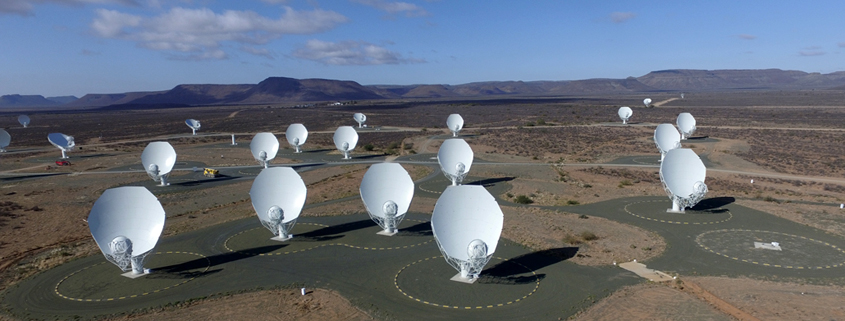
\includegraphics[width=0.5\textwidth]{images/MeerMeer.jpg}
    \caption{Subset of MeerKAT radio telescope in the Karoo, a semi-desert region of South Africa [SKA, South Africa]}
  \label{images/MeerKAT}
\end{figure}

The SKA is an international project to build the world's largest radio telescope array. When complete, it will be a radio telescope with an aperture of up to a million square meters. This powerful, sensitive instrument represents the advance in astronomy, engineering, research and  development to construct a unique scientific instrument \citep{skatelescope}. Two sites chosen for the construction of this tremendous instrument, one of them being the Karoo wilderness of South Africa, where the 64-dish telescope (MeerKAT), a pathfinder to the SKA phase 1, is being constructed \ref{images/MeerKAT}, while the other site is in the Murchison region of Western Australia \citep{hall2008square}.  

When the SKA is complete, it will be a sophisticated instrument to view and track a bevy of cosmic wonders, including objects and events that were too dim or distant for modern astronomers' sky-gazing forebears. This instrument will be far faster ($10^6\times$) than any system currently available, and image the sky in sensitivity ($100\times$) and detail never before achieved \citep{skatelescope}.

\subsection{Big data challenges in radio astronomy}

Astronomy has been among the first scientific disciplines to experience a flood of data. The upcoming SKA is expected to produce terabytes of complex data every hour. The term complex applies both the data that consists of many separate datasets in a large number of different quantities or huge amount of data. This exponential growth in data illustrated in Figure \ref{datagrowth.png} is pushing the requirements for data storage and analysis to the boundaries. The volume and variety of data obtained from the SKA telescope will outstrip the capacity of manual analysis, and in some cases also exceed the capacity of conventional databases currently existing. In view of these challenges caused by the massive data volume, rates, and complexity from next-generation radio telescopes, it is crucial to develop tools that can address astronomical problems faster than astronomers can analyse, such as artificial intelligence systems or algorithms that can connect large datasets to enable broader and deeper analyses than previously possible \citep{provost2013data}. Making new discoveries and revealing the secrets of the universe may not be as simple as previously envisaged. Gone are the days when astronomers could manually detect or notice something odd in their tables or graphs by just browsing through them \citep{RayNorris}. The circumstances of the high volume and speed of data produced by the new, sophisticated astronomical instruments are a great challenge to humans interms of making unexpected discoveries. We wish to make use of computational machinery to
find useful patterns in digital data, and translate these patterns into information that can be used to solve various complex problems, hence machine learning \citep{ball2010data}. This learning must be returned in a useful manner to a human investigator, which will ideally result in human learning \citep{ball2010data}.